\scanpage{47}
\mspage{3)}
% archive sheet number: 46
qui forment un groupoïde \deleted{\unsure{MD}}. $\mathrm{Grbip}$ ou $(\unsure{\mathrm{Grabipond}|\mathrm{Grbipond}})$

% slanted
\margin{pas assez précis comme donnée. La pondération d'une arête doit être remplacée par celle d'un pol. comb. $\unsure{T_{a}}$ avec $\unsure{\omega(T_{a})\simeq\omega(a)}$}
Objets : graphes \inserted{finis} $(S,\vec A,\sigma,o)$ \inserted{+ structure suppl.} (pouvant avoir des sommets isolés, des boucles fermées, a fortiori plusieurs arêtes entre deux sommets, et aussi des ``\uline{arêtes} libres'' correspondant aux pts fixes de $\sigma$)

$S,\vec A$ (ens. fini\unsure{s}) \inserted{(``sommets'', ``\unsure{arcs}'')}, $\sigma:\vec A\mathbin{-}\vec A$ involution, $o:\vec A\to S$ appl. ``origine''. On se donne de plus
\margin{j'ai indiqué une pondération des sommets, mais pas des arêtes}
\figure{
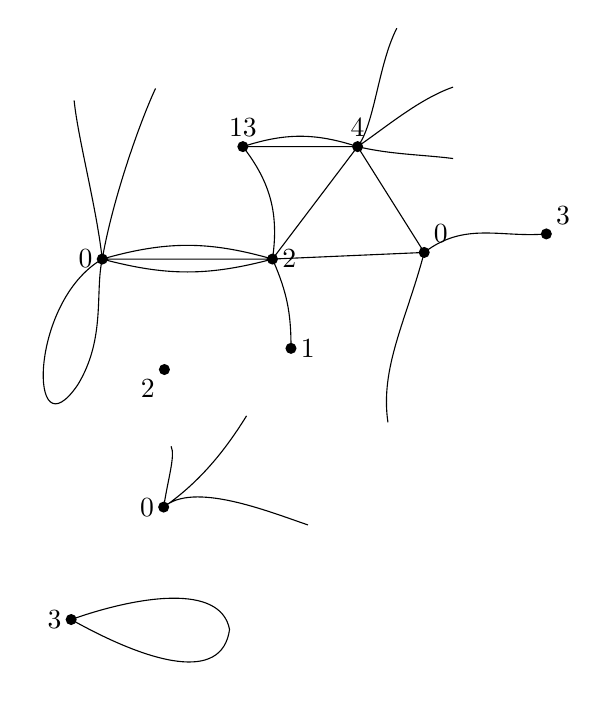
\begin{tikzpicture}[x=.94cm,y=.84cm]
\coordinate (a) at (0,0);
\coordinate (b) at (2.3,0);
\coordinate (c) at (1.9,1.7);
\coordinate (d) at (3.45,1.7);
\coordinate (e) at (4.35,.1);
\coordinate (f) at (6,.38);
\coordinate (g) at (2.55,-1.35);
\draw (a) -- (b) (a) to[bend left=16] (b) (a) to[bend right=15] (b);
\draw (a) .. controls (-1,-.65) and (-1,-3) .. (-.33,-1.9) .. controls (.05,-1.2) and (-.10,-.5) .. (a);
\draw (a) .. controls (-.08,.8) and (-.33,1.83) .. (-.38,2.4);
\draw[thin] (a) .. controls (.14,.9) and (.5,2.05) .. (.72,2.58);
\draw (b) to[bend right=23] (c) (c)--(d) (c) to[bend left=18] (d)
      (b)--(d)--(e)--(b) (b) to[bend left=12] (g);
\draw (d) .. controls (3.68,2.03) and (3.73,2.95) .. (3.98,3.49)
      (d) .. controls (3.83,1.99) and (4.28,2.42) .. (4.74,2.60)
      (d) .. controls (3.9,1.58) and (4.32,1.58) .. (4.74,1.52);
\draw (e) .. controls (4.9,.57) and (5.38,.32) .. (f)
      (e) .. controls (4.11,-.92) and (3.75,-1.64) .. (3.86,-2.47);
\foreach \p/\pos/\weight in {a/left/0,b/right/2,c/above/13,d/above/4,e/above right/0,f/above right/3,g/right/1}
  \fill (\p) circle (2pt) node[\pos] {$\weight$};
\fill (.84,-1.67) circle (2pt) node[below left] {$2$};
\coordinate (h) at (.83,-3.75);
\draw (h) .. controls (.89,-3.31) and (.99,-2.97) .. (.93,-2.83)
      (h) .. controls (1.36,-3.34) and (1.7,-2.82) .. (1.95,-2.37)
      (h) .. controls (1.23,-3.36) and (2.23,-3.81) .. (2.78,-4.02);
\fill (h) circle (2pt) node[left] {$0$};
\coordinate (k) at (-.42,-5.45);
\draw (k) .. controls (.49,-5.09) and (1.6,-4.9) .. (1.72,-5.60)
          .. controls (1.62,-6.41) and (.65,-6.12) .. (k);
\fill (k) circle (2pt) node[left] {$3$};
\end{tikzpicture}
}
\diagram{
\begin{tikzcd}[ampersand replacement=\&]
S\arrow[r,"\deleted{\unsure{g}}\,\unsure{\gamma|g}"] \& \mathbb N
\end{tikzcd}
}
(application ``genre'' ou ``poids'')
\diagram{
\begin{tikzcd}[ampersand replacement=\&]
\deleted{\unsure{\vec A|\widetilde A}}=\unsure{A_\ell|\vec A_\ell}\arrow[r,"\deleted{\unsure{\rho|p}}\,\unsure{r}"] \& \mathbb N
\end{tikzcd}
}
(application \deleted{\unsure{indice de marquage|rigidification}} ``indice de rigidification'')
\deleted{\unsure{déf.} ``\illegible{3}'' $\vec A/\sigma$ \unsure{aux faux sommets} \illegible{1} ``\unsure{vrais sommets}''}

\deleted{Ou encore, posant $\widetilde S=S\amalg A_\ell$, (identifié à l'ens de \uline{tous} les ``sommets'', ``\deleted{\unsure{vrais}}\inserted{\uline{\unsure{marqués|vrais}}}'' (i.e. $\in S$) et ``libres'' (i.e. \unsure{correspondant} aux $\unsure{a\in A_\ell}$) du graphe), l'on donne}
\diagram{
\begin{tikzcd}[ampersand replacement=\&]
\deleted{\widetilde S}\arrow[r,"\deleted{\pi}","\times"description] \& \deleted{\mathbb N}
\end{tikzcd}
}
(\uline{pondération} du graphe)

\margin{$\widetilde S=S\amalg\deleted{\unsure{\widetilde A_\ell}}A_\ell$ \deleted{\illegible{1}}}
\margin{$\widetilde A=\vec A/\sigma=A\amalg A_\ell$}
\diagram{
\begin{tikzcd}[ampersand replacement=\&]
\vec A\arrow[d,"\deleted{\unsure{\pi}}"]=
\& \underset{\vec A\setminus\vec A^\sigma}{\vec A_0}\arrow[d,"\mathrm{deg}\,2"]\amalg
\& \underbrace{\vec A_\ell}_{\vec A^\sigma}\arrow[d,"\mathrm{deg}\,1"]\\
\widetilde A= \& A\amalg \& A_\ell
\end{tikzcd}
}
\margin{Ordre d'un sommet $\,\sigma(s)=\underbrace{\sigma_\ell(s)}_{\substack{\text{correspond}\\\text{aux ``trous''}\\\text{ou cercles}\\\text{de recollage}}}+\sigma_0(s)$}

La donnée du \uline{graphe} sous-jacent à un graphe \deleted{\unsure{MD}}\inserted{bip.} revient à celle du graphe ``ordinaire'' correspondant (sans d'arêtes libres, i.e. où $\sigma$ opère sans pts fixes), i.e.
\[
(S,(\vec A\setminus\vec A^\sigma),\,\sigma|(\vec A\setminus\vec A^\sigma),\,o|\vec A\setminus\vec A^\sigma)),
\]
\uline{plus} un ensemble \inserted{fini} $A_\ell$ (\deleted{\unsure{sommets}}\inserted{arêtes} libres) \deleted{\unsure{ou} ``\unsure{sommets-trous}''} et une application
\[
A_\ell\longrightarrow S
\]
\uline{Flèches}\quad les iso. de telles structures
